\graphicspath{{chapters/images/01/}}
%TODO Fix image sizes, captions and references 

\chapter{High-throughput biological data}
  High-throughput techniques, ofter referred to as \textbf{omic techniques}, are a way to collect extensive, comprehensive, quantitative and large scale data on a certain aspect of a biological system. The main omics data types are genomics, transcriptomics, proteomics, metabolomics; each of them possesses specific individual technologies and methods. 

  \section{Required biological background}
    It is assumed that you posses some amount of knowledge regarding the following topics:
    \begin{itemize}
      \item Molecular biology of the cell (cell types and characteristics)
      \item Molecular components of the cell (mainly proteins and nucleic acids)
    \end{itemize}

  \section{Genomics}
    \textbf{Genomics} refers to the study of the genome, which is the entire DNA (or RNA in some bacteria and viruses) content of a cell. The focus is generally on the variation of the genome of an individual (or a group of individuals) compared to a reference genome (a sequence that is shared by most individuals of a scpecies). Particularly important is the study of \textbf{SNPs} (Single Nucleotide Polymorphisms) which allows to retrieve information such as philogenetics, disease predisposition, forensic applications (individual recognition, paternity testing...) and many others. SNPs can be studied either via \textbf{DNA microarrays}, which are economic since they target only specific regions of the genome where the presence of SNPs is known, or via \textbf{whole genome sequencing}, which is more expensive but gives information. 
    
    \subsection{Genomic wide association studies}
      \textbf{Genome Wide Association Studies} (GWAS) are studies where many genetic markers are studied across the genome a population in orded to try and correlate them to specific conditions (mainly predisposition and presence of disease).

      \begin{figure}[h]
      \caption{Manhattan plot: Mahnattan plots are a common way to represent GWAS results}
      \centering
      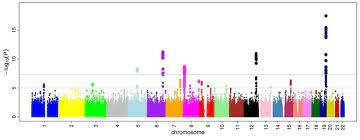
\includegraphics[width=0.6\textwidth]{ManhattanPlot.jpg}
      \end{figure}


  \section{Transcriptomics}
    The \textbf{transcriptome} is the collection of mRNA species/transcripts in a cell at a given time. It can provide a lot of information on cell state, growth conditions and many others, which is why it is heavily studied; moreover transcriptomics is \textbf{robust}, relatively \textbf{cost effective} and \textbf{user friendly}.
    
    \subsection{Microarrays}
      \textbf{Microarrays} can be used to measure levels of mRNA in a high-throughput fashion.
      Roughly, a microarry workflow can be summarized as:
      \begin{itemize}
        \item Extract RNA content from cells
        \item Obtain fluorescence-marked cDNA
        \item Hybridize the cDNA with the DNA probes on the chip 
        \item Wash chip to remove non-hybridized cDNA
        \item Record output fluorescent signal
        \item Normalize the result:
        \begin{itemize}
          \item If using a 2 color microarray (red-marked test sample, green marked control sample), you obtain the fold expression of the transcript compared to the reference (red = overexpressed, yellow = same expression level, green = underexpressed)
          \item If using a single color microarray (only marked test sample) the output can be normalized in various ways, generally substracting the signal of aspecific probes (of the 20-25 bases a couple of them are mismatched, to test for aspecific interaction)
        \end{itemize}
        Further normalization steps may be required
        % \cite{smythNormalizationCDNAMicroarray2003}
        \item Analyze the output
      \end{itemize}

      \begin{figure}[h]
      \caption{Microarray output: Genes with different expressions can be visualized, each column is a sample and each row is one of the 25 genes. The colour represents the level of expression}
      \centering
      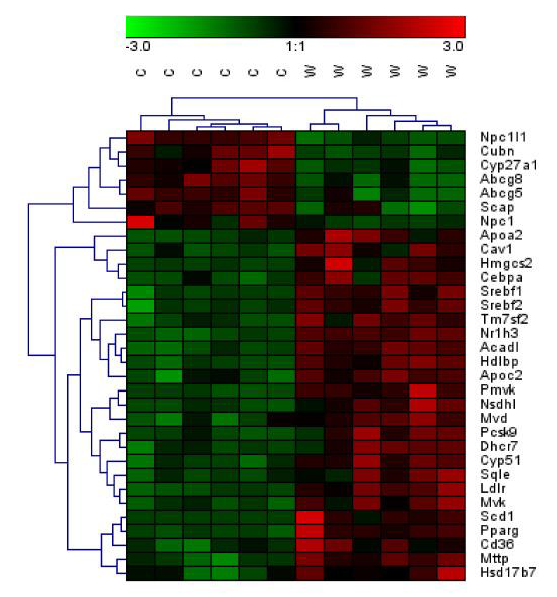
\includegraphics[width=0.6\textwidth]{MicroRNAresults.PNG}
      \end{figure}

    \subsection{Next generation sequencing}
      \textbf{Next generation sequencing} (NGS) is another way to analyize the transcriptome; each mRNA species in each sample is broken into fragments, and all fragments are sequenced base by base. The current technologies manage to sequence small pieces of RNA, around 250 bases. By using overlapping ends of the fragments, we can reassamble RNAs. A higher amount of fragments grants an higher coverage. This method allows \textbf{massively parallel sequencing}, \textbf{sequencing of both known and unknown transcipt} (no probe requirement), detecting transcripts in a \textbf{high dynamic range} (up to $10^6$ copies)

      \begin{figure}[h]
      \caption{NGS flowchart}
      \centering
      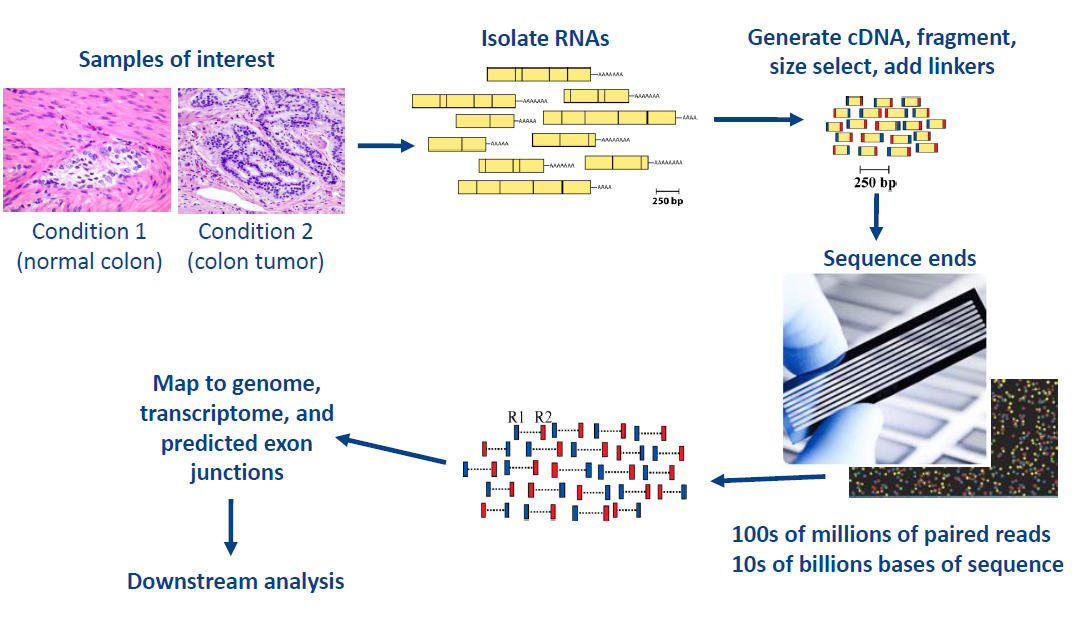
\includegraphics[width=0.6\textwidth]{TranscriptomicsNextGenSeq.PNG}
      \end{figure}

    \subsection{RNA-seq pipeline}
      After obtaining the raw sequencing results, the RNA-seq pipeline uses some other resources, namely input files (reference genome, gene annotation) and programmes (some accessed through cloud to speed up data analysis), to obtain polished information and results.

      \begin{figure}[h]
      \caption{RNA-seq pipeline}
      \centering
      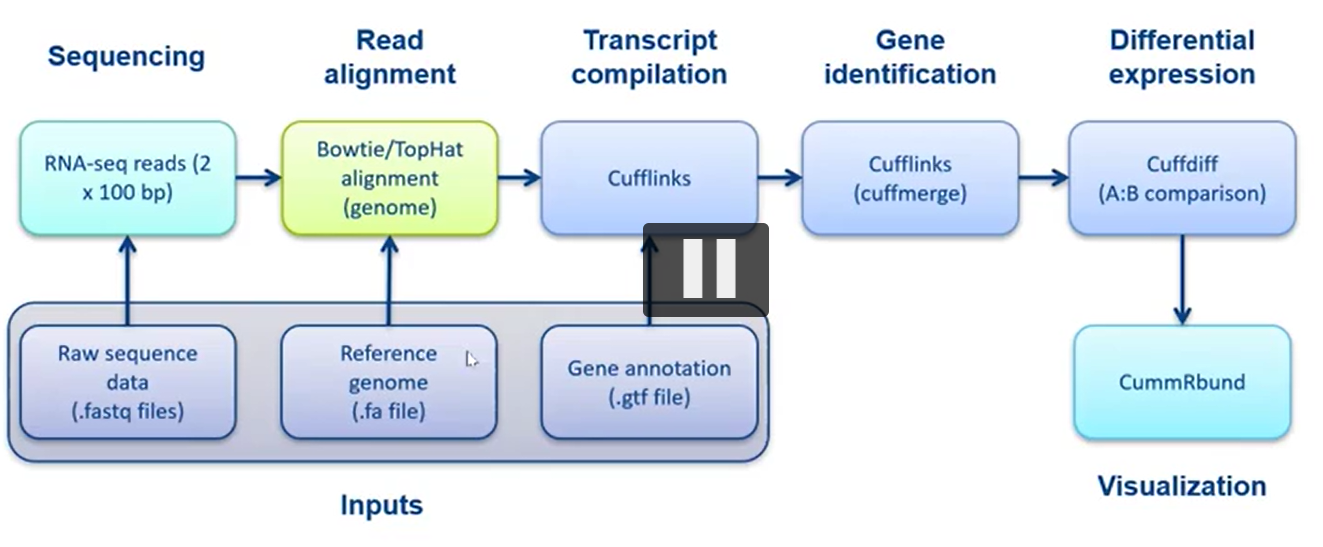
\includegraphics[width=0.6\textwidth]{RNAseqpipeline.PNG}
      \end{figure}

    \subsection{Microarrays vs sequencing}
      Overall, microarrays are more economic but can only give information on transcripts for which a specific probe exists on the chip. They allow to obtain differential expression studies but not absolute quantification. Sequencing is more costly, but unbiased and higher-throughput; moreover it allows further analysis, such as mapping and absolute quantification.

  \section{Proteomics}
    The \textbf{proteome} is the set of all proteins produced under a given set of conditions. The analysis of the proteome, called proteomics, has countless applications. Proteomic techniques allow for high-throughput analysis of protein content, yet again the throughput is significantly lower than transcriptomic techiques: this is because proteins are more complex than nucleic acids, both in structure and sequence, and they do not have a convenient 1:1 pairing pattern. For this reasons, proteomic techniques usually rely on other physical characteristics, mainly \textbf{mass} and \textbf{charge}.

    \subsection{2D gel electrophoresis}
      Standard gel electrophoresis separates proteins based on their size (varying the crosslinking rate of the polyacrylamide net); this method has very limited resolution (it is influenced by many factors, such as denaturation, SDS coating, fragmentation...).
      2D gel electrophoresys partially increments the resolution since it separate proteins based on both weight and charge.
      The standard protocol for 2D gel electrophoresis consists of:
      \begin{itemize}
        \item Protein extraction, purification and usually denaturation
        \item First dimension electrophoresis: proteins migrate in a low density gel in which molecules have been placed to create a pH gradient. The proteins distribute along the gradient solely because of their charge (regardless of mass)
        \item Second dimension electrophoresis: the first dimension gel is placed at the edge of a regular polyacrylamide gradient gel, which allows to separate the molecules by weight. 
        \item Coloration and acquisition of gel signal
        \item The result is a sort of map, with increasing pH value from left to right and decreasing weight from top to bottom.
      \end{itemize}
      These maps can be then compared either with maps from other samples (to identify differences) or with databases to identify the proteins spots. Notice that this procedure does not technically identify univocally the protein and thus, if required, you might have to cut the protein spot from the gel and procede with further analysis. Another significant problem with this technique is the need for large amounts of samples to have significant signal levels.

      \begin{figure}[h]
      \caption{Isoelectric focusing: separation of proteins in a pH gradient}
      \centering
      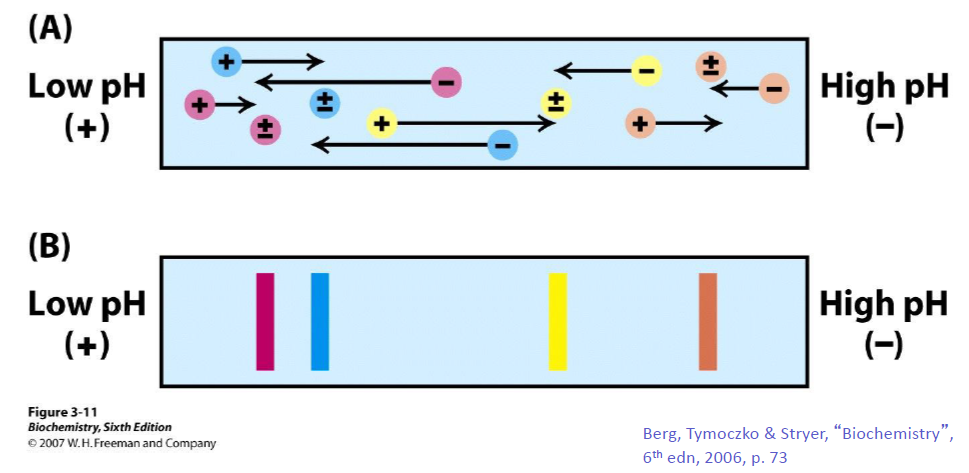
\includegraphics[width=0.6\textwidth]{IsoelectricProteinSeparation}
      \end{figure}

    \subsection{Liquid chromatography/mass spectrometry}
      Mass spectrometry consists of a plethora of techniques that allow to separate molecules based on their mass to electrical charge ratio. This technique allows for high-throughput identification of proteins (without need for further analysis). The main limitation of mass spectrometry is the need for highly purified protein extracts (and thus labour intensive procedures) since it is highly susceptible to contaminants; for this reason the protein extract is usually purified and diluted using liquid chromatography and the output is analyzed via mass spectrometry (from which the name liquid chromatography/mass spectrometry or LC-MS for short). Another big advantage of this technique is the very low amount of sample required (some $\mu g$ of purified proteins are enough). Mass spectrometry does not allow for absolute quantification but only relative quantification (due to peptide volatilization and other factors). LC-MS can usually identify up to about 1000 proteins per sample (more realistically around 600-700 due to dynamic range issues). LC-MS can be used to study also post-traslation modifications (such as phosphorilation).

    \subsection{Protein arrays}
      \textbf{Protein arrays} are conceptually similar to DNA arrays, but instead of DNA probes they use \textbf{aptamers}, which are oligonucleotides or peptide molecules designed to uniquely bind to a specific molecule. Proteins bind the aptamers and a fluorescent signal is used for detection. This method is easy and cheap, but it measures a low amount of proteins and only proteins for which an aptamer was found. It is still an emergent technology.
      % \cite{neaguProteinMicroarrayTechnology2019}.

      \begin{figure}[h]
      \caption{Protein array}
      \centering
      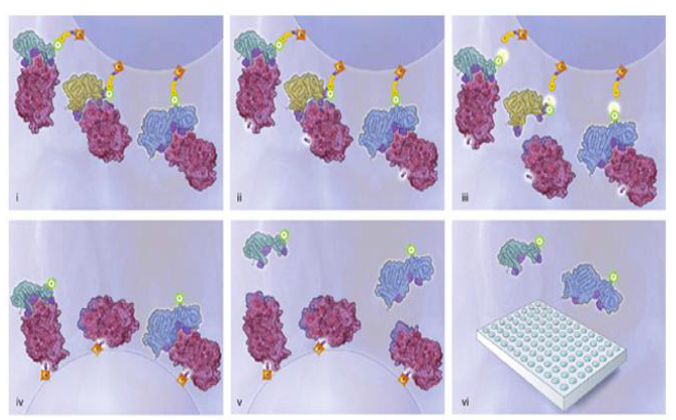
\includegraphics[width=0.6\textwidth]{ProteinArray}
      \end{figure}
    
    \subsection{Proteomics vs transcriptomics}
      Both proteomics and transcriptomics are very powerful techniques. In general transcriptomics is cheaper, more robust and user-friendly, while proteomics pose some more limitations, namely due to protein purification and stability. Both techniques keep being developed since they provide different informations, for example transcriptomics allows to study non-coding RNAs while proteomics allows to study post-translational modifications (the opposite in not true).

  \section{Metabolomics} 

    \textbf{Metabolomics} is a field of life science research that uses high-throughput technologies to identify and/or characterize all the small molecules or metabolites in a given cell, tissue or organism (the so called metabolome). There are two main approaches in metabolomics:
    \begin{itemize}
      \item Quantitative methods: quantitatively identify target metabolites in a sample
      \item Chemometric methods: profiling samples based on metabolites in them
    \end{itemize}
    These approaches can be useful, for instance, to early detection and diagnosis of diseases, since certain metabolites correlate do higher risk of certain pathologies.
  
  \section{Other high-throughput data sources}
    Countless other sources of high-throughput data exist and many more are becoming viable. 

    \subsection{Microbiome}
      With the term \textbf{microbiome} we collectively refer to all the microbes in the human body, whether they are bacteria, fungi, protozoa, viruses or other. This heterogeneous population is of interested since it is highly represented in most regions of our body; the role of microbes is important since they contribute to some physiological functions of the organism (gut microbes), they can cause pathologies when deregulated, their populations show differences among individual hosts.
      (\textit{To go into more detail, please refer to the "Computational Microbial Genomics Notes - Segata" available \href{https://github.com/giacThePhantom/computational-microbial-genomics}{\textbf{here}}})

    \subsection{Epigenomics}
      \textbf{Epigenetics} is the study of heritable changes in gene activity that are not caused by changes in the DNA sequence. Some mechanisms that produce such changes are \textbf{DNA methylation} and \textbf{histone modification}. Both mechanisms alter how genes are expressed without altering the underlying DNA sequence.
      %TODO potentially add more

      \begin{figure}[h]
      \caption{Examples of epigenetic modifications}
      \centering
      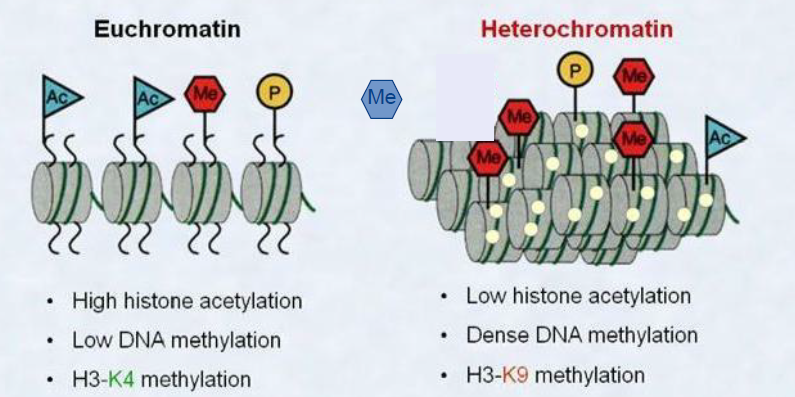
\includegraphics[width=0.6\textwidth]{EuEteroChromatin}
      \end{figure}

    \subsection{Micro RNAs}
      Micro RNAs, or miRNAs, are a family (around 1000 in humans) of short (20-22 bases) non-coding RNAs which affect mRNA translation and therefore protein expression. They are produced as precursors in the nucleus, then when they find and pair with their target sequence, they recruit cellular machinery that activates them and causes transcript degradation. miRNAs can be isolated from total RNA and can be profiled to get information on genes that are currently regulated.
      %TODO potentially add more

    \subsection{Interactome}
      The \textbf{interactome} of a protein is the set of molecules (generally other proteins) that interact with that specific protein (therefore we usually talk about protein-protein interaction). Studying the interactome of a protein can help understand its function and possible ways to modulate its activity. There are databases for interactomes. Interactomes are generally shown in 3D graphs, with nodes representing proteins and lines representing connections between them.  
      %TODO potentially add more

\chapter{Clinical trial study design}
  
  \section{Required background}
    Some basic knowledge regarding cell lines, immortalized cell lines, model organisms, human studies and their pros and cons are required. \textit{This section might be expanded more clearly in the future}.

    %TODO Decide if actually expanding it or not
